\section{Homework 4}
\subsection{Exercise 4.11}
The task is to formulate different norms as LPs
\subsubsection{Part a}
Minimizing $\| Ax-b \|_\infty$. This norm is the same as the maximum entry of $Ax-b$
\begin{equation}
  \min \| Ax-b \|_\infty = \min \max \{A_i x - b_i, i=1,\dots,n\} 
\end{equation}

\begin{equation}
  \begin{aligned}
    \min z \\
    \text{subject to } z \geq A_i x - b_i, i = 1,\dots, n
  \end{aligned}
\end{equation}

\subsubsection{Part b}
Minimizing$\| Ax-b \|_1$. The $l_1$ norm is equal to
\begin{equation}
  \sum_i |A_i x - b_i |
\end{equation}
where $A_i$ is the $i$-th row of the matrix $A$. We can turn this into
\begin{equation}
  \begin{aligned}
    \text{minimize } \sum_i |z_i| \\ 
    \text{subject to } z_i = A_i x - b_i; i = 1,\dots,m
  \end{aligned}
\end{equation}
Removing the absolute value
\begin{equation}
  \begin{aligned}
    \text{minimize } \sum_i z_i \\ 
    \text{subject to } A_i x - b_i \leq z_i; i = 1,\dots,m \\
    b_i - A_i x \leq z_i; i = 1,\dots,m 
  \end{aligned}
\end{equation}
Vector notation
\begin{equation}
  \begin{aligned}
    \text{minimize } \textbf{1}^T z \\ 
    \text{subject to } A x - b \preceq z\\
    b - A x \preceq z
  \end{aligned}
\end{equation}

\subsubsection{Part c}
Minimizing $\| Ax-b \|_1$ subject to $\| x \|_\infty \leq 1$
\begin{equation}
  \begin{aligned}
    \text{minimize } \textbf{1}^T z \\ 
    \text{subject to } A x - b \preceq z\\
    b - A x \preceq z \\
    \| x \|_\infty \leq 1
  \end{aligned}
\end{equation}
Expanding the $l_\infty$ norm

\begin{equation}
  \begin{aligned}
    \text{minimize } \textbf{1}^T z \\ 
    \text{subject to } A x - b \preceq z\\
    b - A x \preceq z \\
    x  \preceq \textbf{1} \\
    -x \preceq \textbf{1}
  \end{aligned}
\end{equation}

\subsubsection{Part d}
Minimizing $\| x \|_1$ subject to $\| Ax -b \|_\infty \leq 1$
\begin{equation}
  \begin{aligned}
    \text{minimize } \textbf{1}^T z \\ 
    \text{subject to } x \preceq z\\
    - x \preceq z \\
    A x - b \preceq \textbf{1}\\
    b - A x \preceq \textbf{1}\\
  \end{aligned}
\end{equation}

\subsubsection{Part e}
Minimizing $\| Ax-b \|_1 + \| x \|_\infty$
\begin{equation}
  \begin{aligned}
    \text{minimize } \textbf{1}^T z + s \\ 
    \text{subject to } x \preceq s\\
    - x \preceq s \\
    A x - b \preceq z\\
    b - A x \preceq z\\
  \end{aligned}
\end{equation}



\subsection{Exercise 4.16}
The minimum fuel optimal control problem as an LP. First, starting with what was given in the problem with minimal changes:
\begin{equation}
  \begin{aligned}
    \text{minimize } \sum_{t=0}^{N-1} f(u(t)) \\
    \text{subject to } x(t+1) = Ax(t) + bu(t) \\
    x(N) = x_{des} \\ 
    x(0) = 0
  \end{aligned}
\end{equation}
With the fact that 
\begin{equation}
  f(u) = 
  \begin{cases} 
      |u| & |u| \leq 1 \\
      2|u| -1 & |u|> 1
  \end{cases}
\end{equation}
This is not a linear equation, but we can manipulate it and find that this is equivalent to
\begin{equation}
  f(y) = 
  \begin{cases} 
      y & y \leq 1 \\
      2y -1 & y> 1
  \end{cases}
\end{equation}
\begin{equation}
  \text{subject to } -y \leq u \leq y
\end{equation}
This function can be linearized by introducing a new variable as the function and using inequalities.
\begin{equation}
  \begin{aligned}
    f(z) = z \\
    \text{subject to } z \geq y \\
    z \geq 2y-1 \\
    -y \leq u \leq y
  \end{aligned}
\end{equation}

This can be brought to the original problem and formulated as the below LP
\begin{equation}
  \begin{aligned}
    \text{minimize }\textbf{1}^T z \\
    \text{subject to } x(t+1) = Ax(t) + bu(t) \\
    x(N) = x_{des} \\
    x(0) = \textbf{0}  \\
    z \geq y \\
    z \geq 2y -1 \\
    -y \leq u(t) \leq y
  \end{aligned}
\end{equation}


\subsection{Exercise 4.29}
Verifying convexity or quasiconvexity of the problem 
\begin{equation}
  \begin{aligned}
    \text{maximize } \textbf{prob}(c^T x \geq \alpha) \\
    \text{subject to } Fx \leq g, Ax = b
  \end{aligned}
\end{equation}
In this problem, the constraints are both affine so the whole problem is convex as long as the objective function is convex.

\subsection{Exercise 4.30}
For this problem, the costs are defined as 
\begin{equation}
  \begin{aligned}
    c_1 = \frac{\alpha_1 T r}{w} \\
    c_2 = \alpha_2 r \\
    c_3 = \alpha_3 r w \\
    c_T = \sum_{i=1}^{3}c_i
  \end{aligned}
\end{equation}
As stated, this problem can be modeled as 
\begin{equation}
  \begin{aligned}
    \text{maximize } \alpha_4 T r^2 \\
    \text{subject to } \frac{\alpha_1 T r}{w} + \alpha_2 r + \alpha_3 r w \leq C_{max} \\
    T_{min} \leq T \leq T_{max} \\
    r_{min} \leq r \leq r_{max} \\
    w_{min} \leq w \leq w_{max} \\
    w \leq 0.1r
  \end{aligned}
\end{equation}

This is equivalent to the below geometric program
\begin{equation}
  \begin{aligned}
    \text{minimize } \frac{1}{\alpha_4} T^{-1} r^{-2} \\
    \text{subject to } \frac{\alpha_1 T r w^{-1} + \alpha_2 r + \alpha_3 r w}{C_{max}}\leq  1\\
    \frac{1}{T_{max}} T  \leq 1 \\
    T_{min} T^{-1}\leq 1 \\
    \frac{1}{w_{max}} w  \leq 1 \\
    w_{min} w^{-1} \leq 1 \\
    \frac{1}{r_{max}} r  \leq 1 \\
    r_{min} r^{-1}\leq 1 \\
    10wr^{-1} \leq 1
  \end{aligned}
\end{equation}

\subsection{Exercise 5.1}
Looking at the optimization problem

\begin{equation}
  \begin{aligned}
    \text{minimize } x^2 +1 \\
    \text{subject to } (x-2)(x-4) \leq 0
  \end{aligned}
\end{equation}
\subsubsection{Part a}
The feasible set is the interval from $[2,4]$. The optimal value is $5$ and the optimal solution is $x=2$ 

\subsubsection{Part b}
Solving for the lagrangian
\begin{equation}
  \begin{aligned}
    L(\lambda, x) = x^2+1 + \lambda (x-2)(x-4) \\
    g(\lambda) = \inf_x L(\lambda, x) \\
    \frac{d }{d x} x^2+1 + \lambda(x-2)(x-4) = 2x + \lambda(2x -6) \\
    2x + \lambda 2x = 6\lambda \\
    x = \frac{3\lambda}{1+\lambda} \\ 
    g(\lambda) = (\frac{3\lambda}{1+\lambda})^2 + 1 + \lambda( (\frac{3\lambda}{1+\lambda}) -2 )(\frac{3\lambda}{1+\lambda} -4)
  \end{aligned}
\end{equation}

\begin{figure}[htbp]
  \centerline{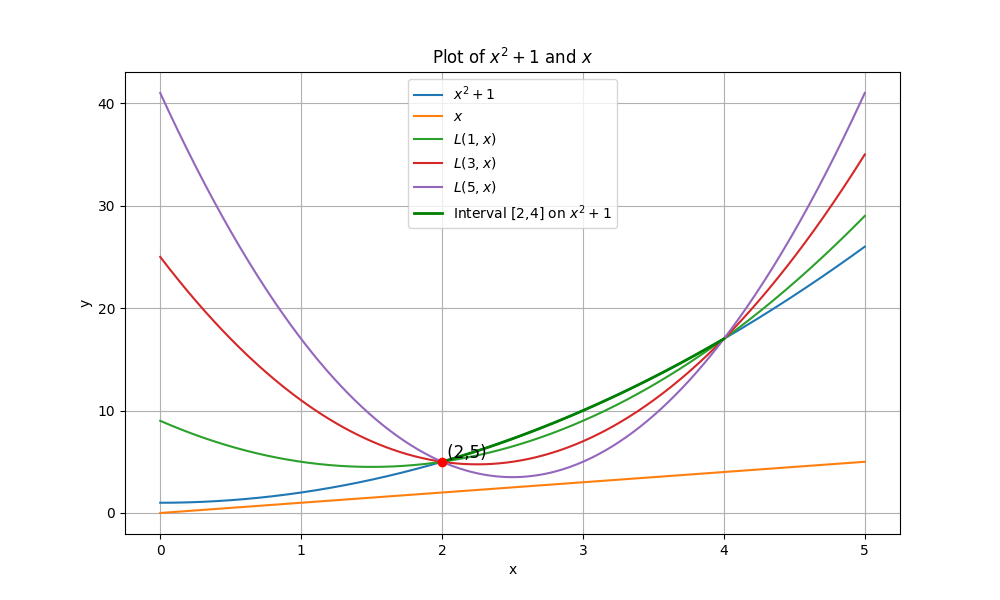
\includegraphics[width=0.75\textwidth]{hw4/5_1_part_b_1.png}}
  \caption{Plot of the feasible set with lagrangian}
  \label{fig:5_1_b_1}
\end{figure}

\begin{figure}[htbp]
  \centerline{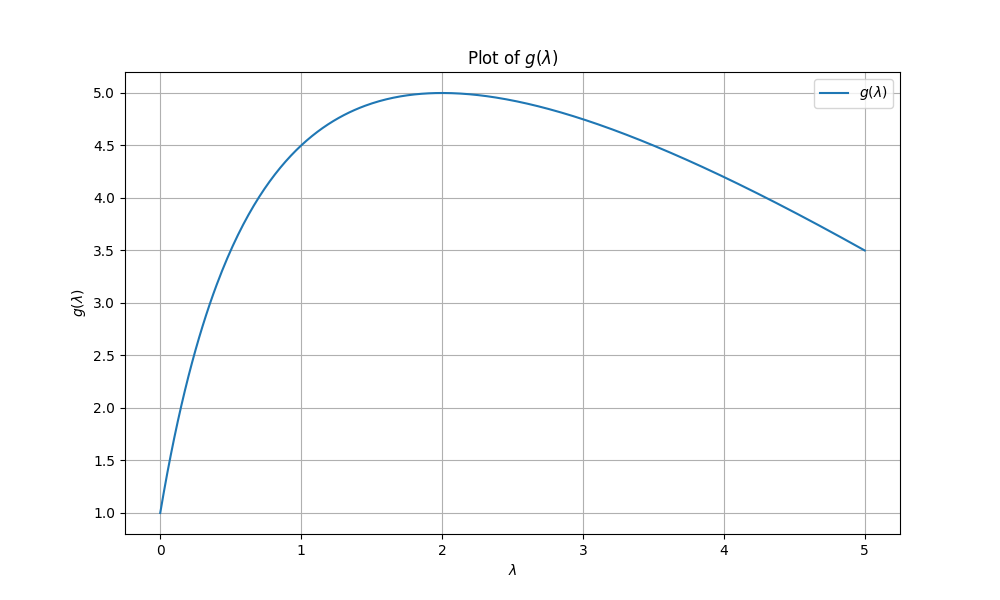
\includegraphics[width=0.75\textwidth]{hw4/5_1_part_b_2.png}}
  \caption{Plot of the lagrangian dual}
  \label{fig:}
\end{figure}
